%% BioMed_Central_Tex_Template_v1.06
%%                                      %
%  bmc_article.tex            ver: 1.06 %
%                                       %

%%IMPORTANT: do not delete the first line of this template
%%It must be present to enable the BMC Submission system to
%%recognise this template!!

%%%%%%%%%%%%%%%%%%%%%%%%%%%%%%%%%%%%%%%%%
%%                                     %%
%%  LaTeX template for BioMed Central  %%
%%     journal article submissions     %%
%%                                     %%
%%          <8 June 2012>              %%
%%                                     %%
%%                                     %%
%%%%%%%%%%%%%%%%%%%%%%%%%%%%%%%%%%%%%%%%%


%%%%%%%%%%%%%%%%%%%%%%%%%%%%%%%%%%%%%%%%%%%%%%%%%%%%%%%%%%%%%%%%%%%%%
%%                                                                 %%
%% For instructions on how to fill out this Tex template           %%
%% document please refer to Readme.html and the instructions for   %%
%% authors page on the biomed central website                      %%
%% http://www.biomedcentral.com/info/authors/                      %%
%%                                                                 %%
%% Please do not use \input{...} to include other tex files.       %%
%% Submit your LaTeX manuscript as one .tex document.              %%
%%                                                                 %%
%% All additional figures and files should be attached             %%
%% separately and not embedded in the \TeX\ document itself.       %%
%%                                                                 %%
%% BioMed Central currently use the MikTex distribution of         %%
%% TeX for Windows) of TeX and LaTeX.  This is available from      %%
%% http://www.miktex.org                                           %%
%%                                                                 %%
%%%%%%%%%%%%%%%%%%%%%%%%%%%%%%%%%%%%%%%%%%%%%%%%%%%%%%%%%%%%%%%%%%%%%

%%% additional documentclass options:
%  [doublespacing]
%  [linenumbers]   - put the line numbers on margins

%%% loading packages, author definitions

\documentclass[twocolumn]{bmcart}% uncomment this for twocolumn layout and comment line below
%\documentclass{bmcart}

%%% Load packages
\usepackage{amsthm,amsmath}
\usepackage{siunitx}
\usepackage{mfirstuc}
%\RequirePackage{natbib}
\usepackage[colorinlistoftodos]{todonotes}
\RequirePackage{hyperref}
\usepackage[utf8]{inputenc} %unicode support
%\usepackage[applemac]{inputenc} %applemac support if unicode package fails
%\usepackage[latin1]{inputenc} %UNIX support if unicode package fails
\usepackage[htt]{hyphenat}

\usepackage{array}
\newcolumntype{L}[1]{>{\raggedright\let\newline\\\arraybackslash\hspace{0pt}}p{#1}}

%%%%%%%%%%%%%%%%%%%%%%%%%%%%%%%%%%%%%%%%%%%%%%%%%
%%                                             %%
%%  If you wish to display your graphics for   %%
%%  your own use using includegraphic or       %%
%%  includegraphics, then comment out the      %%
%%  following two lines of code.               %%
%%  NB: These line *must* be included when     %%
%%  submitting to BMC.                         %%
%%  All figure files must be submitted as      %%
%%  separate graphics through the BMC          %%
%%  submission process, not included in the    %%
%%  submitted article.                         %%
%%                                             %%
%%%%%%%%%%%%%%%%%%%%%%%%%%%%%%%%%%%%%%%%%%%%%%%%%


%\def\includegraphic{}
%\def\includegraphics{}

%%% Put your definitions there:
\startlocaldefs
\endlocaldefs


%%% Begin ...
\begin{document}

%%% Start of article front matter
\begin{frontmatter}

\begin{fmbox}
\dochead{Report from 2015 OHBM Hackathon (HI)}

%%%%%%%%%%%%%%%%%%%%%%%%%%%%%%%%%%%%%%%%%%%%%%
%%                                          %%
%% Enter the title of your article here     %%
%%                                          %%
%%%%%%%%%%%%%%%%%%%%%%%%%%%%%%%%%%%%%%%%%%%%%%

\title{NiftyView: A Zero-Footprint Web Application for viewing DICOM and NIfTI
files}
\vskip2ex
\projectURL{Project URL: \url{http://www2.hawaii.edu/\%7Eweiran/NiftyView.html}}

\author[
addressref={aff1},
corref={aff1},
email={weirandeng@gmail.com}
]{\inits{WD} \fnm{Weiran} \snm{Deng}}

%%%%%%%%%%%%%%%%%%%%%%%%%%%%%%%%%%%%%%%%%%%%%%
%%                                          %%
%% Enter the authors' addresses here        %%
%%                                          %%
%% Repeat \address commands as much as      %%
%% required.                                %%
%%                                          %%
%%%%%%%%%%%%%%%%%%%%%%%%%%%%%%%%%%%%%%%%%%%%%%

\address[id=aff1]{%
  \orgname{University of Hawaii John A. Burns School of Medicine, Honolulu, Hawaii,
USA},
  \city{Honolulu},
  %
  %
  \postcode{Hawaii},
  \cny{USA}
}

%%%%%%%%%%%%%%%%%%%%%%%%%%%%%%%%%%%%%%%%%%%%%%
%%                                          %%
%% Enter short notes here                   %%
%%                                          %%
%% Short notes will be after addresses      %%
%% on first page.                           %%
%%                                          %%
%%%%%%%%%%%%%%%%%%%%%%%%%%%%%%%%%%%%%%%%%%%%%%

\begin{artnotes}
\end{artnotes}

%\end{fmbox}% comment this for two column layout

%%%%%%%%%%%%%%%%%%%%%%%%%%%%%%%%%%%%%%%%%%%%%%
%%                                          %%
%% The Abstract begins here                 %%
%%                                          %%
%% Please refer to the Instructions for     %%
%% authors on http://www.biomedcentral.com  %%
%% and include the section headings         %%
%% accordingly for your article type.       %%
%%                                          %%
%%%%%%%%%%%%%%%%%%%%%%%%%%%%%%%%%%%%%%%%%%%%%%

%\begin{abstractbox}

%\begin{abstract} % abstract
	
%Blank Abstract

%\end{abstract}



%%%%%%%%%%%%%%%%%%%%%%%%%%%%%%%%%%%%%%%%%%%%%%
%%                                          %%
%% The keywords begin here                  %%
%%                                          %%
%% Put each keyword in separate \kwd{}.     %%
%%                                          %%
%%%%%%%%%%%%%%%%%%%%%%%%%%%%%%%%%%%%%%%%%%%%%%

%\vskip1ex

%\projectURL{\url{http://www2.hawaii.edu/\%7Eweiran/NiftyView.html}}
%\projectURL{http://www2.hawaii.edu/\%7Eweiran/NiftyView.html}

% MSC classifications codes, if any
%\begin{keyword}[class=AMS]
%\kwd[Primary ]{}
%\kwd{}
%\kwd[; secondary ]{}
%\end{keyword}

%\end{abstractbox}
%
\end{fmbox}% uncomment this for twcolumn layout

\end{frontmatter}

%{\sffamily\bfseries\fontsize{10}{12}\selectfont Project URL: \url{http://www2.hawaii.edu/\%7Eweiran/NiftyView.html}}

%%% Import the body from pandoc formatted text
\section{Introduction}\label{introduction}

The purpose of developing yet another web-based image viewer, NiftyView,
is to use WebGL to take advantage of the parallel computing power in
Graphics Processing Units (GPU) hardware for the acceleration of
rendering and processing of medical images in web applications. Although
several web-based medical image viewers such as
\href{https://github.com/rii-mango/Papaya}{Papaya},
\href{https://brainbrowser.cbrain.mcgill.ca}{BrainBrowser} and
\href{http://slicedrop.com}{Slice:Drop} are currently available, the
slow performance of the web-based applications is still one of the major
limitations of web-based image viewers. NiftyView is a free web
application developed in JavaScript. It has zero footprint; only a web
browser and an Internet connection are needed to run NiftyView. It's
advantageous over conventional desktop applications in that NiftyView
doesn't require installation and constant updates. The current version
supports \href{http://nifti.nimh.nih.gov}{NIfTI} and
\href{http://dicom.nema.org}{DICOM} format. As a minimal image viewer,
it's a convenient tool for users who need a quick and easy tool for
viewing medical images. Currently, the beta version of NiftyView is
freely available at
http://www2.hawaii.edu/\textasciitilde{}weiran/NiftyView.html .

\section{Approach}\label{approach}

NiftyView is developed in JavaScript with
\href{http://jquery.com}{jQuery} for HTML document manipulation and
event handling, \href{http://jqueryui.com}{jQueryUI} for user interface,
and \href{https://github.com/chafey/dicomParser}{DicomParser} for
parsing DICOM files. It's compatible with popular web browsers including
Internet Explorer, Safari, Firefox, and Opera. Either DICOM or NIfTI
files can be loaded by dragging files into the browser window. Loaded
images can be displayed in single-slice mode or tiled mode. After
loading, images are automatically arranged according to the scan IDs for
DICOM files and the file name for NIfTI files, respectively. Current
functions include image zooming and adjustment of image brightness and
contrast. The number of image columns can be adjusted in the tiled mode
to maximize the use of the display space. The contrast and brightness of
images can be adjusted by clicking and holding the right mouse button or
using a double slider widget in the horizontal tool bar at the top of
the window. For proof-of-concept, functions such as pixel windowing and
scaling are programmed using WebGL by translating the arithmetic
operations in image processing to 3D graphics primitives using WebGL's
programmable shaders. The pixel values of an image is loaded into a
frame buffer. A vertex shader is programmed to define vertices
corresponding to the coorddinates of the image, and a fragment shader is
programmed to perfrom arithmetic operations, which are performed in
parallel to a massive number of image pixels.

\section{Results}\label{results}

See Figures 1 and 2.

\begin{figure}[h!]
  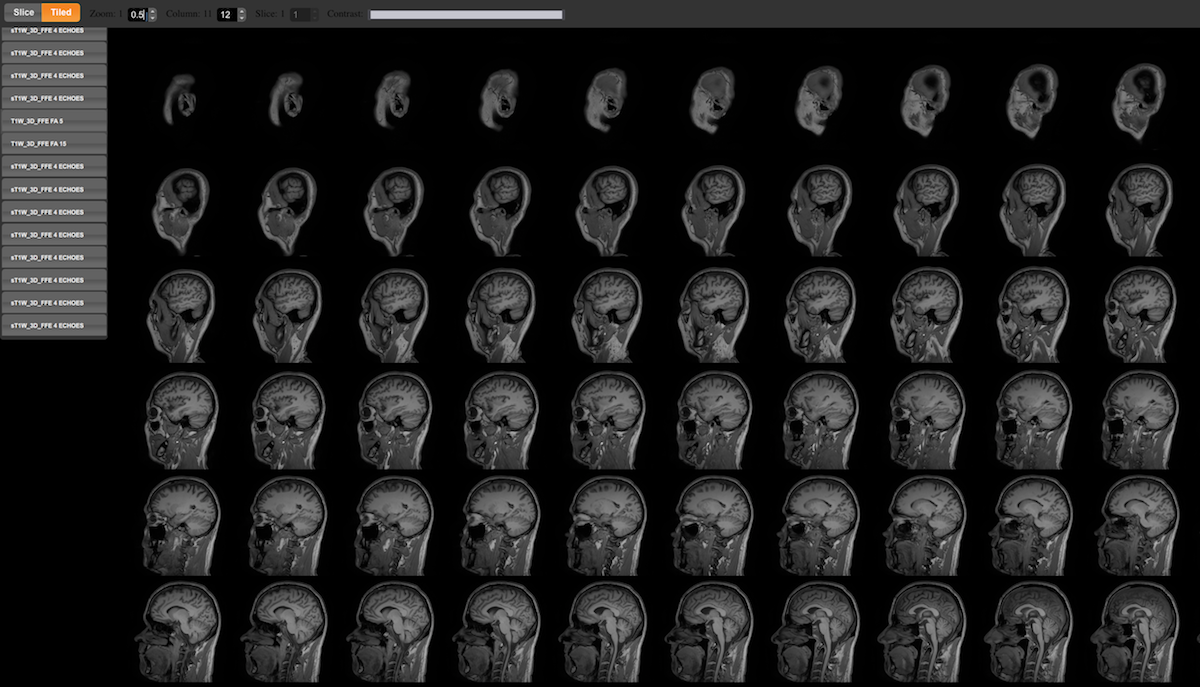
\includegraphics[width=.47\textwidth]{niftyview_ui}
  \caption{\label{centfig}
  A few sagittal MRI images displayed in titled mode after loaidng approximately 1,500 DICOM files from 11 MRI scans. It took approximately ten seconds to load all the DICOM files into NiftyView. The images are organized into different vertical tabs by the sequence names stored in the DICOM files.}
\end{figure}

\begin{figure}[h!]
  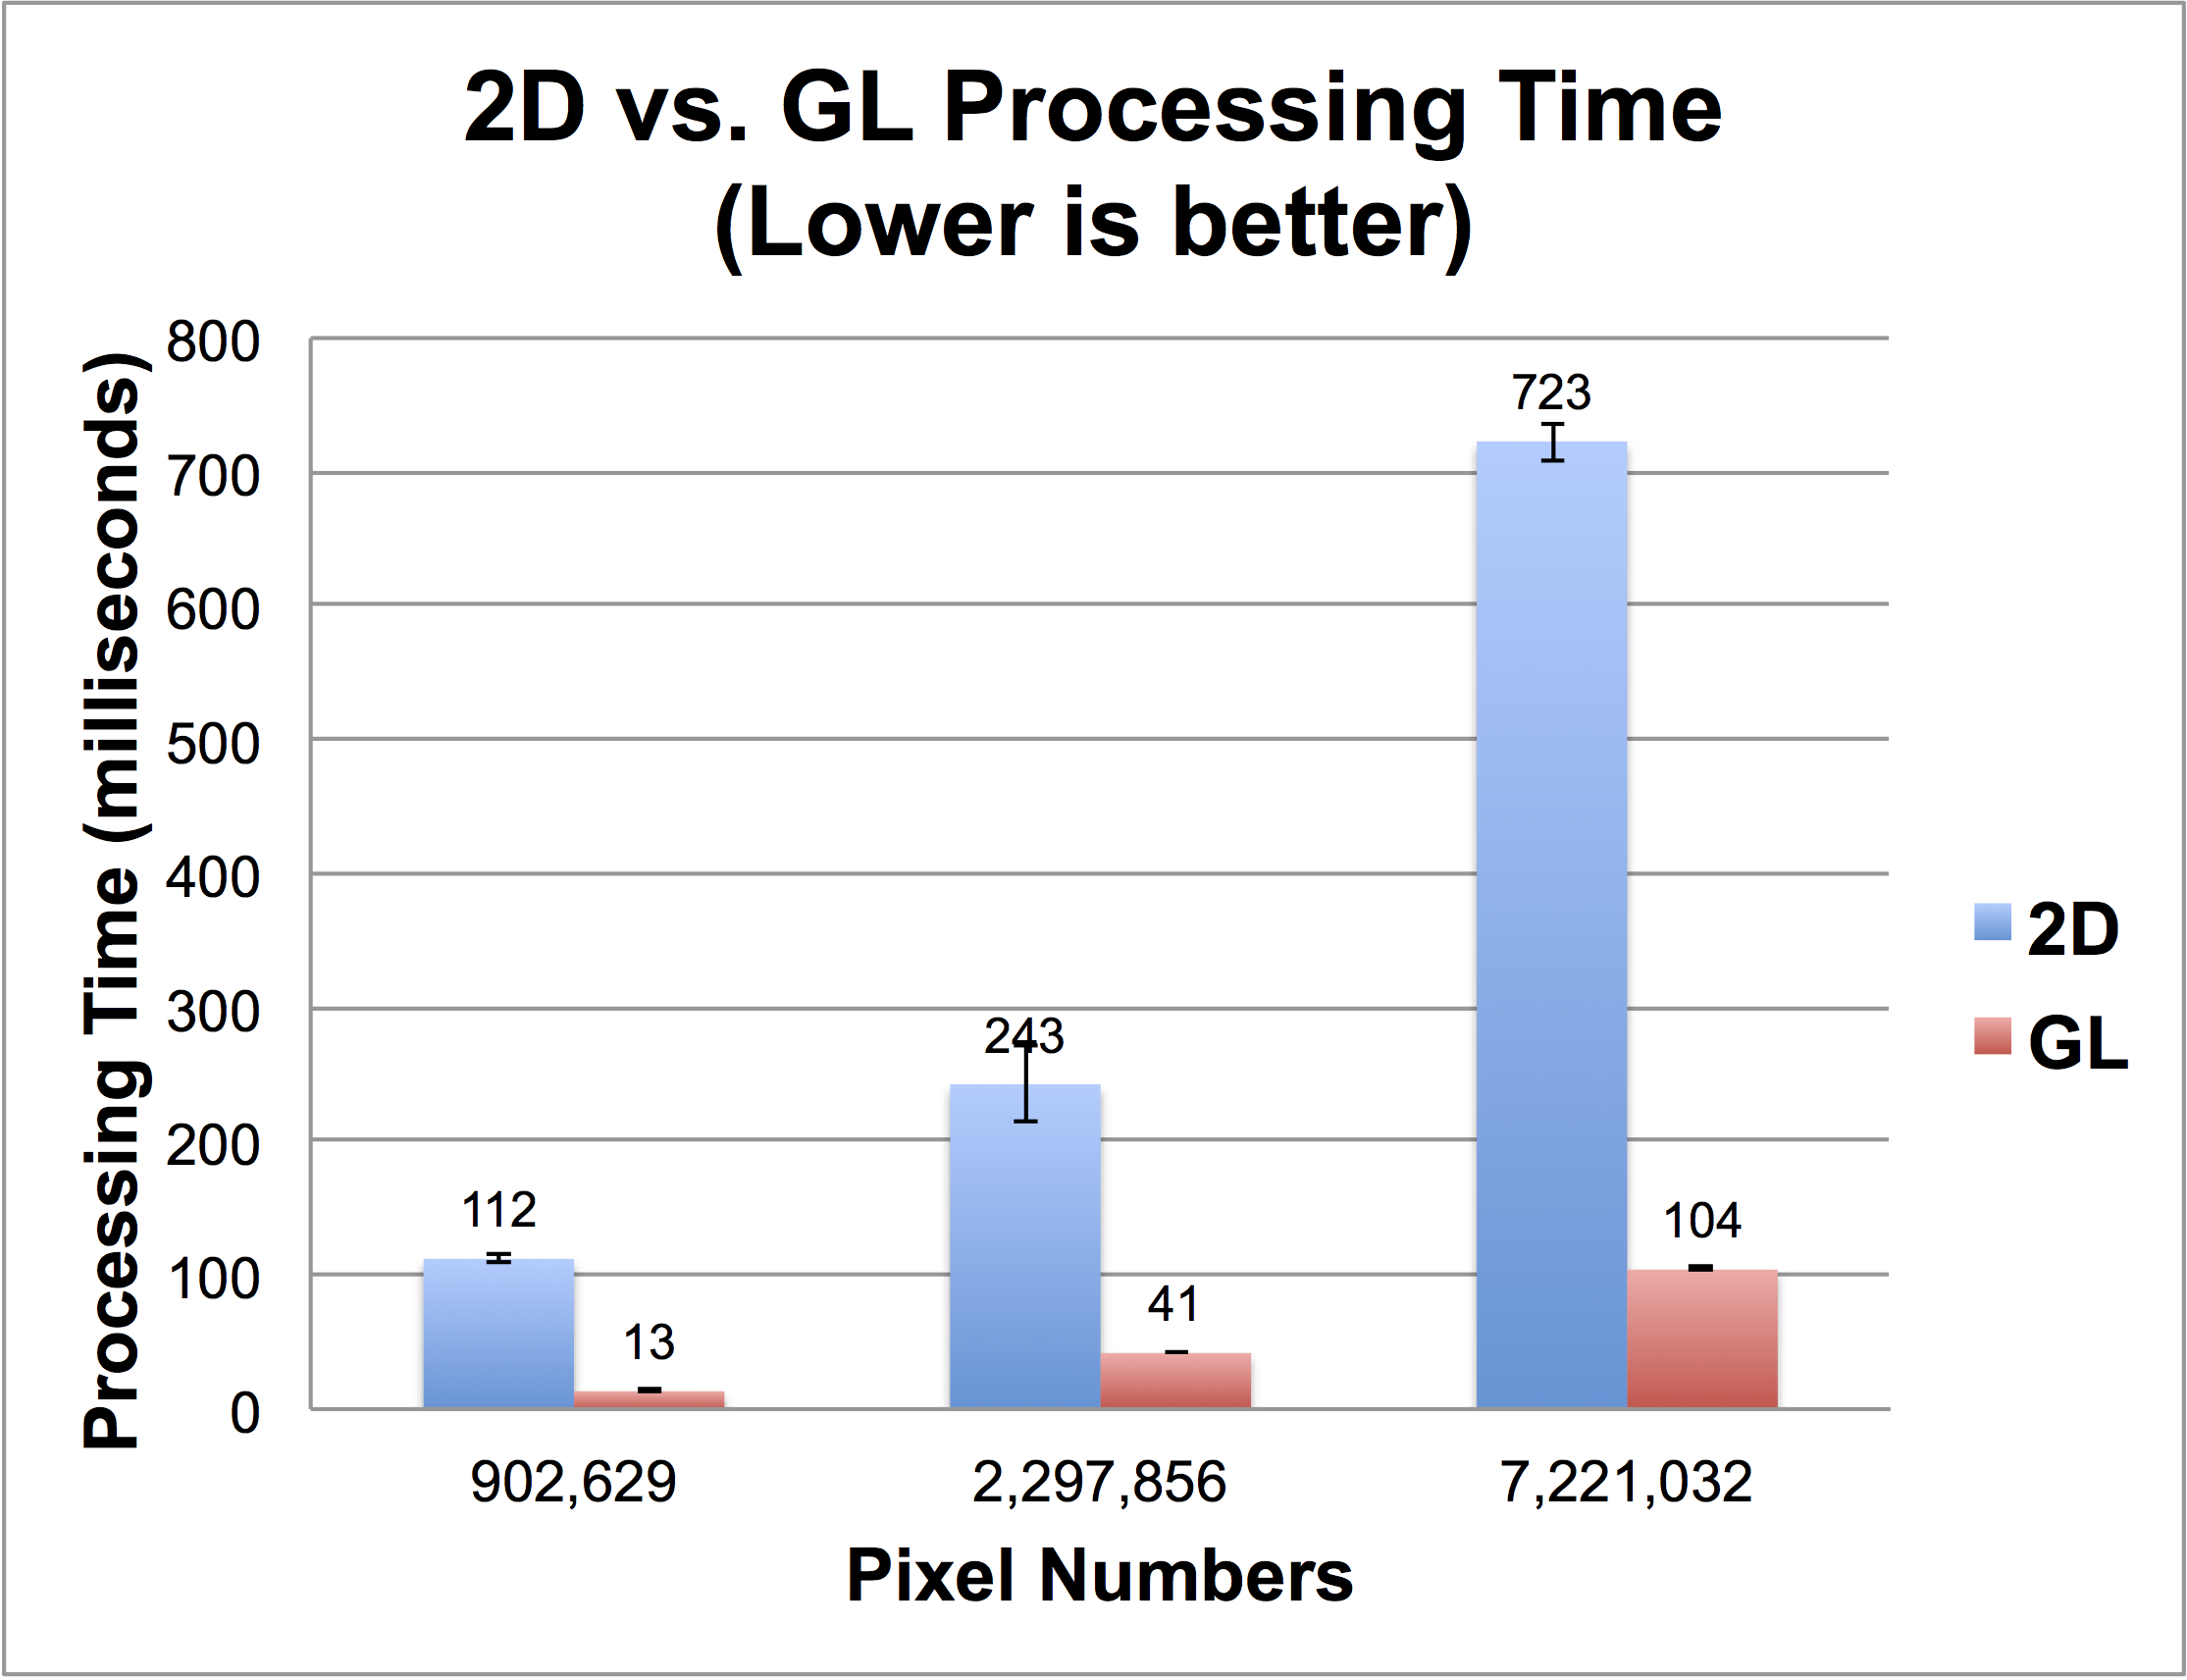
\includegraphics[width=.47\textwidth]{2d_vs_gl_processing_time.png}
  \caption{\label{centfig}
  Image of WebGL vs. Canvas Comparison. Shows a comparison of processing time as a function of the number of image pixels in JavaScript(blue) and WebGL (red). WebGL shows a factor of six to eight accelerations. }
  \end{figure}

\section{Discussion}\label{discussion}

One of the major limitations of current web-based image viewers is the
slow performance compared to their desktop counterparts.

There are collective efforts in industry to develop new technologies
such as WebAssmebly and WebGL to narrow this performance gap. The highly
parallel nature in processing image pixels independently allows the use
of WebGL to achieve a signficant speedup, as shown in this abstract.
Currently, there are several similar existing web applications such as
Papaya, BrainViewer, and slicedrop.com, which are more mature and offer
varieties of features. However, the main goal of the continuing effor in
the development of NiftyView is to achieve a high performance for image
processing using GPU via WebGL. NiftyView has a minimal boilerplate and
can handle a large number of files with relative ease. Future work will
be focused on developing a WebGL-accelerated version, adding more image
processing features, and adding support of accessing files stored in
HIPAA (Health Insurance Portability and Accountability Act) compliant
cloud storage servies such as Box and Amazon S3. The stable version of
NiftyView will be released under a General Public License that allows
end users to freely run, modify, and share the program.

\section{Conclusion NiftyView is a free and convenient web application
for}\label{conclusion-niftyview-is-a-free-and-convenient-web-application-for}

quick and easy viewing of NIfTI and DICOM medical images. We have shown
that a factor of six to eight acceleration can be achieved using WebGL
for image processing.

%%%%%%%%%%%%%%%%%%%%%%%%%%%%%%%%%%%%%%%%%%%%%%
%%                                          %%
%% Backmatter begins here                   %%
%%                                          %%
%%%%%%%%%%%%%%%%%%%%%%%%%%%%%%%%%%%%%%%%%%%%%%

\begin{backmatter}

\section*{Availability of Supporting Data}
More information about this project can be found at: \url{http://www2.hawaii.edu/\%7Eweiran/NiftyView.html}. Further data and files supporting this project are hosted in the \emph{GigaScience} repository REFXXX.

\section*{Competing interests}
None

\section*{Author's contributions}
\emph{Author's contributions statement is missing.}

\section*{Acknowledgements}
\emph{Acknowedgements section is missing.}

  
  
%%%%%%%%%%%%%%%%%%%%%%%%%%%%%%%%%%%%%%%%%%%%%%%%%%%%%%%%%%%%%
%%                  The Bibliography                       %%
%%                                                         %%
%%  Bmc_mathpys.bst  will be used to                       %%
%%  create a .BBL file for submission.                     %%
%%  After submission of the .TEX file,                     %%
%%  you will be prompted to submit your .BBL file.         %%
%%                                                         %%
%%                                                         %%
%%  Note that the displayed Bibliography will not          %%
%%  necessarily be rendered by Latex exactly as specified  %%
%%  in the online Instructions for Authors.                %%
%%                                                         %%
%%%%%%%%%%%%%%%%%%%%%%%%%%%%%%%%%%%%%%%%%%%%%%%%%%%%%%%%%%%%%

% if your bibliography is in bibtex format, use those commands:
\bibliographystyle{bmc-mathphys} % Style BST file
\bibliography{brainhack-report} % Bibliography file (usually '*.bib' )

\end{backmatter}
\end{document}
